\documentclass[12pt]{report}
\usepackage[utf8]{inputenc}
\usepackage[russian]{babel}
%\usepackage[14pt]{extsizes}
\usepackage{listings}

% Для листинга кода:
\lstset{language=Go,
	basicstyle=\ttfamily\scriptsize,
	keywordstyle=\color{blue}\ttfamily,
	stringstyle=\color{red}\ttfamily,
	commentstyle=\color{green}\ttfamily}

% Для измененных титулов глав:
\usepackage{titlesec, blindtext, color} % подключаем нужные пакеты
\definecolor{gray75}{gray}{0.75} % определяем цвет
\newcommand{\hsp}{\hspace{20pt}} % длина линии в 20pt
% titleformat определяет стиль
\titleformat{\chapter}[hang]{\Huge\bfseries}{\thechapter\hsp\textcolor{gray75}{|}\hsp}{0pt}{\Huge\bfseries}

%отступы по краям
\usepackage{geometry}
\geometry{verbose, a4paper,tmargin=2cm, bmargin=2cm, rmargin=1.5cm, lmargin = 3cm}
% межстрочный интервал
\usepackage{setspace}
\onehalfspacing
\usepackage{float}
% plot
\usepackage{pgfplots}
\usepackage{filecontents}
\usepackage{amsmath}
\usepackage{tikz,pgfplots}
\usetikzlibrary{datavisualization}
\usetikzlibrary{datavisualization.formats.functions}

\usepackage{graphicx}
\graphicspath{{src/}}
\DeclareGraphicsExtensions{.pdf,.png,.jpg}

\usepackage{geometry}
\geometry{verbose, a4paper,tmargin=2cm, bmargin=2cm, rmargin=1.5cm, lmargin = 3cm}
\usepackage{indentfirst}
\setlength{\parindent}{1.4cm}

\usepackage{titlesec}
\titlespacing{\chapter}{0pt}{12pt plus 4pt minus 2pt}{0pt}
\usepackage{indentfirst}
\setlength{\parindent}{1.4cm}

\usepackage{amsmath}

\begin{document}
%\def\chaptername{} % убирает "Глава"
\tableofcontents
\setcounter{page}{2}

\newpage
\chapter*{Введение}
\addcontentsline{toc}{chapter}{Введение}

Задачи данной лабораторной работы:
\begin{itemize}
	\item Изучить метод Пикара;
	\item реализовать метод Пикарда, явный и неявный методы Эйлера, метод Рунге-Кутты второго порядка точности для решения уровнения $y'(x) = x^2 + y^2$;
	\item сравнить методы между собой.
\end{itemize}
\chapter{Аналитическая часть}
В данной части будут рассмотрены теоретические основы методов Пикара, явного и неявного методов Эйлера. 

\section{Постановка задачи} 
Пусть поставлена задача Коши:
\begin{equation*}
	\begin{cases}
	u'(x) = f(x, u(x))\\
	u(x_0) = u_0 \\
	x_0 \leq x \leq x_l
	\end{cases}
\end{equation*}
\section{Метод Пикара}
Данный метод является представителем класса приближенных методов решения.
Идея метода чрезвычайно проста и сводится к процедуре последовательных приближений для решения интегрального уравнения, к которому приводится исходное дифференциальное уравнение.

Проинтегрируем выписанное уравнение

\begin{equation}
	u(x) = u_0 + \int_{x_0}^{x} f(t,u(t))dt
\end{equation}

Процедура последовательных приближений метода Пикара реализуется согласно следующей схеме.
\begin{equation}
y_s(x) = u_0 + \int_{x_0}^{x} f(t,y_{s-1}(t))dt
\end{equation}
причем $y_0(t) = u_0$

\section{Явный метод Эйлера}
Самый простой метод решения уровнения - дискретизация расчетного интервала и замена производной в левой части $\frac{du(x)}{dt}$	разностным аналогом. Для некоторой i-ой точки сетки разностная производная определяется следующим образом:
\begin{equation}
\frac{du(t_i)}{dt} \approx \frac{y_{i+1} - y_i}{h}
\end{equation}
Для того, чтобы схема имела простое решение, правую часть уравнения возьмем в той же точке $t_i$:
\begin{equation}
\frac{y_{i+1} - y_i}{h} = f(t_i, y_i)
\end{equation}
Таким образом, мы сразу получаем рекуррентную формулу определения нового значения y в точке $t_{i+1}$, т.е. $y_{i+1}$ по значению y в точке $t_{i+1}$. Это значение обозначим как $y_{i}$, а $y_{i+1}$ запишем как:
\begin{equation}
y_{i+1} = y_i + h \cdot f(x_i,y_i)
\end{equation}
\section{Неявный метод Эйлера}
\begin{equation}
y_{i+1} = y_i + h \cdot f(x_i+1,y_i+1)
\end{equation}
Геометрическая интерпретация  одного шага этого метода заключается в том, что решение на отрезке $[t_i;t_{i+1}]$ аппроксимируется касательной $y = y_{i+1} + y'(t_{i+1})(t-t_{i+1})$, проведенной в точке $(t_{i+1},y_{i+1})$ к интегральной кривой, проходящей через эту точку.
\chapter{Технологическая часть}

\section{Выбор ЯП}
В качестве языка программирования был выбран golang.
Время работы алгоритмов было замерено с помощью time. 
\section{Листинг кода алгоритмов}
В данном разделе будут приведены листинги кода решения методом Пикара (Листинг \ref{picard}) и Эйлера (Листинг \ref{euler})
\begin{lstlisting}[label=picard,caption = Метод Пикара, language = go]

func picard(x float64, n int)float64{
	u0 := 0.0
	answer := 0.0
	poly := make(map[int]float64)
	curr := make(map[int]float64)
	poly[2] = 1.0
	var res float64
	for i:=0;i<n;i++{
		curr = poly_pow(curr)
		curr[2] = 1.0
		curr, res = integrate(curr, 0.0, x)
		answer = u0 + res
	}
	return answer
}

//add term to polinomial
func add(poly map[int]float64, term *term)map[int]float64{
	if _, ok := poly[term.pow]; ok{
		poly[term.pow] += term.coef
	}else{
		poly[term.pow] = term.coef
	}
	return poly
}

//multiply two terms and write to polinomial
func mult(poly map[int]float64, term1, term2 *term)map[int]float64{
	to_add := multterm(term1, term2)
	add(poly, to_add)
	return poly
}

//multiply two terms and return result
func multterm(term1, term2 *term)*term{
	res := term{term1.coef*term2.coef, term2.pow+term1.pow}
	return &res
}

//squaring a polinomial
func poly_pow(poly map[int]float64) map[int]float64{
	res := make(map[int]float64)
	for i, j := range poly{
		for k, z := range poly{
			mult(res, &term{j, i}, &term{z,k})
		}
	}
	return res
}

func integrate(poly map[int]float64, x0, x float64) (map[int]float64, float64){
	var answer float64
	res := make(map[int]float64)
	for i, j := range poly{
		integr := term{j, i+1}
		integr.coef *= 1.0/float64(integr.pow)
		res[integr.pow] = integr.coef
		answer += integr.coef*math.Pow(x, float64(integr.pow)) -
			 integr.coef*math.Pow(x0, float64(integr.pow))
	}
	return res, answer
}
\end{lstlisting}

\newpage
\begin{lstlisting}[label=euler,caption = Явный и неявный методы Эйлера, language = go]
func euler_explicit(xn float64, n int)float64{
	h := xn / float64(n)
	y:=0.0 
	x:=0.0
	for i:=0; i<=n;i++{
		y = y + h*f(x, y)
		x+=h
	}
	return y
}
func euler_implicit(xn float64, n int)float64{
	h := xn / float64(n)
	y:=0.0 
	x:=0.0
	var a, b, c, dis, x1 float64
	for i:=0;i<=n;i++{
		a = 1; b = -1.0/h; c = 1.0/h*y+(x+h)*(x+h)
		dis = D(a, b, c)
		if dis>=0{
			x1 = (-b - math.Sqrt(dis))/2/a
		}
		y = x1
		x+=h
	}
	return y
}
\end{lstlisting}

\begin{lstlisting}[label=euler,caption = Метод Рунге-Кутты, language = go]
func runge_kutta(xn float64, n int)float64{
	h := xn / float64(n)
	alpha := 0.5
	y := 0.0
	x := 0.0
	
	for i:=0; i<n;i++{
		y += h * ( (1- alpha) * f(x,y) + alpha * f(x+h/(2*alpha), y+(h/2*alpha)*f(x,y)) )
		x+=h
	}
	_ = x
	return y
}
\end{lstlisting}

\chapter{Примеры работы программы}
\begin{figure}[h]
	\centering{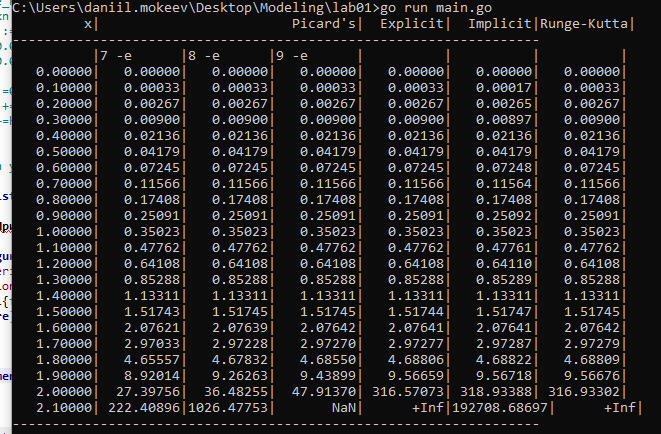
\includegraphics[scale = 0.9]{7-8-9.png}}
	\caption{Приблежения 7,8,9}
	\label{fig:f_p}
\end{figure}

\begin{figure}[h]
	\centering{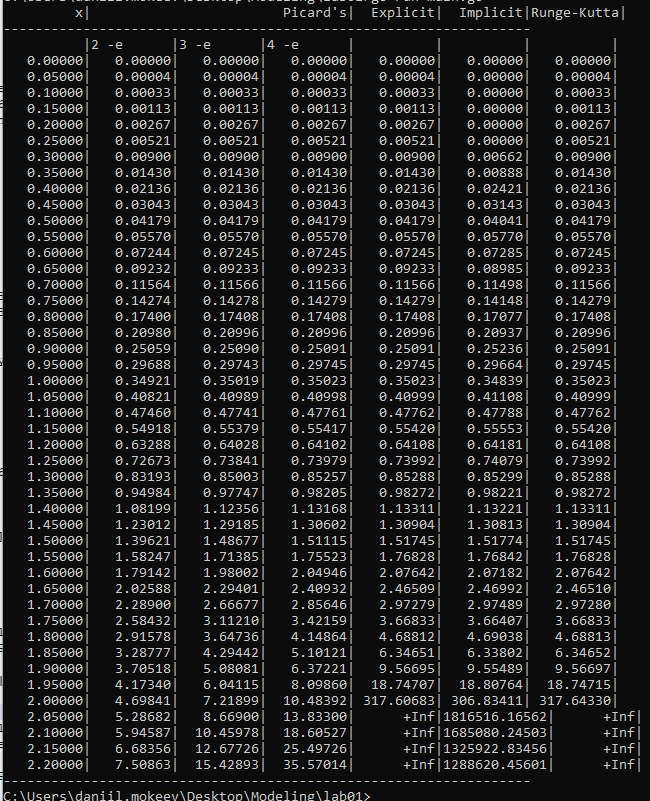
\includegraphics[scale = 0.9]{2-3-4.png}}
	\caption{Приблежения 2,3,4}
	\label{fig:f_p}
\end{figure}

\chapter{Ответы на контрольные вопросы}

\section*{Укажите интервалы значений аргумента, в которых можно считать решением заданного уравнения каждое из первых 4-х приближений Пикара. Точность результата оценивать до второй цифры после запятой. Объяснить свой ответ.}
Каждое новое приблежение метода Пикара увеличивает точность решения. Для оценки точности n-ого приблежения можно сравнить его со следующим.
\begin{equation}
	|y_{n+1} - y_n| < \epsilon
\end{equation}
где $\epsilon$ - заданная погрешность

Для точности $\epsilon = 0.01$:
\begin{itemize}
	\item 1-ое приблежение $x \in [0;0.69]$
	\item 2-ое приблежение $x \in [0;1.11]$
	\item 3-е приблежение $x \in [0;1.35]$
	\item 4-е приблежение $x \in [0;1.51]$
\end{itemize}

\section*{Пояснить, каким образом можно доказать правильность полученного результата при фиксированном значении аргумента в численных методах}
Для подтверждения правильности полученного результата можно уменьшать значение шага при вычислении метода. Так как точность численных методов зависит от значения шага, если при уменьшении этого значения результат будет меняться на значение меньшее, чем $\epsilon$, это значение можно считать верным.

Так как из-за ограний ЭВМ нельзя уменьшать шаг до предельно малых значений, реальное решение можно получить только с заданной погрешностью.

\section*{Из каких соображений выбирался корень уравнения в неявном методе?}
Выбирался меньший корень для минимизации ошибки.


\section*{Каково значение функции при x=2, т.е. привести значение u(2).}
Значения приведены в примерах работы программы.
\end{document}

